\chapter{背景}\label{chap:background}

第二章介绍了本工作所涉及到的一些工程技术方面的背景知识,包括Tilelink总线协议,芯片验证的基础知识以及业界常用的UVM验证方法学等。这部分背景知识补齐了一些技术细节,帮助读者更好地理解本工作的后续内容。

\section{TileLink一致性协议}

\subsection{TileLink简介}

TileLink是芯片级的互连标准,为多个主设备提供对内存和其他从设备的一致性的内存映射访问。TileLink作为快速可扩展互连协议,可提供低延迟和高吞吐量的传输。它被设计用于在片上系统(SoC)中连接通用多处理器,协处理器,加速器,DMA引擎以及简单或复杂的设备。
TileLink是类似ARM AXI和ACE的,通用的、支持一致性的总线协议以及互联标准。
TileLink的一些重要特性包括:
\begin{enumerate}
	\item 标准免费开放
	\item 为RISC-V设计,但也支持其他的ISA
	\item 为任意的缓存(如处理器核)或非缓存主设备(如DMA master)提供一致性的内存访问,支持类似MESI的一致性协议
\end{enumerate}

这些重要特性,让TileLink在开源芯片设计中广受欢迎。TileLink相关IP(如CrossBar,Arbiter,SerDes,NoC等)齐全并且很成熟,同时大量的开源芯片设计都使用TileLink总线作为访存接口,如Rocket Chip,Boom等。

为了支持各种不同设备从简单到复杂的访存需求,TileLink规范定义了三种协议兼容级别,这些级别说明了设备必须支持协议的哪个子集,如下表所示。
最简单的是TileLink轻量级不缓存(TL-UL),仅支持简单的内存读写(Get/Put)单个字的操作。它可以用于简单的,只需要单个字读写访问的,如UART之类外设。
接下来最复杂的是TileLink重量级不缓存(TL-UH),它添加了各种Hint(提示),原子操作和突发访问,但不支持一致性缓存。它可以用于稍微复杂一点的,需要较高数据吞吐量,同时又不需要自己硬件上维护一致性的主设备,如ICache,DMA master等。
最后,TileLink缓存(TL-C)是完整的协议,它支持使用一致性的缓存。它可以用于完整的,自己维护硬件一致性的cache,如DCache,L2,L3等各级Cache。

TL-UL和TL-UH中的消息,都是master请求slave执行一些读写预取操作,master没有获取数据块的权限,不要求将数据块的所有权从slave转移到master这边。因此它们常常用于master自己不需要缓存数据块(如DMA engine),或者master自己缓存的数据块是软件维护一致性,不需要硬件维护一致性(例如ICache)的情况。由于master并不请求数据块权限以缓存在本地,所以这些请求被称为uncached请求,这也是两个协议名称中U的由来。

TL-UL,TL-UH和TL-C三种兼容性级别,低级别是高级别的真子集,高级别包含了低级别的所有通道,所有消息(低级别的消息在高级别中功能可能会被扩展)。
兼容性级别越高,支持的消息越来越多,支持的功能越来越强。相应的,master和slave端的实现也就更加复杂。


\begin{center}
\begin{tabular}{|l|l|l|l|}
\hline
                      & \textbf{TL-UL} & \textbf{TL-UH} & \textbf{TL-C} \\ \hline
Read/Write operations & $\checkmark$   & $\checkmark$   & $\checkmark$  \\ \hline
Multibeat messages    & $\checkmark$   & $\checkmark$   & $\checkmark$  \\ \hline
Atomic operations     & $\checkmark$   & $\checkmark$   & $\checkmark$  \\ \hline
Hint operations       & $\times$       & $\checkmark$   & $\checkmark$  \\ \hline
Cache block transfers & $\times$       & $\times$       & $\checkmark$  \\ \hline
Channels B+C+E        & $\times$       & $\times$       & $\checkmark$  \\ \hline
\end{tabular}
\end{table}

我感觉应该把channel,message,transaction合并成一页,然后再把coherence搞一页。
关于tilelink,大家主要要理解啥呢?tilelink有哪些流程,它们走的什么通道。每个通道是用来干啥的,就OK了吧?
其他太过于细节的,其实是不必要的啊。

channel上是message,message构成transaction,transaction支持请求的流程。然后对于这些流程,我们只需要着重介绍read/write,还有cache block transfer就好了吧。
这个应该怎么介绍了呢,自底向上或者自顶向下都是可以的吧。
随便介绍一下就OK了吧。

\subsection{TileLink通道、消息、事务和一致性}

上一节介绍了TileLink的主要特性,这一节主要介绍TileLink的一些技术细节,包括它的通道定义,消息,事务以及如何实现一致性。
这些内容是具有递进关系的。
通道是底层的逻辑链路,通道承载了消息。
消息往往是单向(从master到slave或者从slave到master)的信息流动。例如,读请求消息(从master到slave)或者读数据回复(从slave到master)。
事务是一个最基础的请求流程,例如读和写。多个逻辑上相关的消息一起组成了一个事务,例如,读由读请求和读数据回复组成;写由写请求和写回复组成。
而一致性则是系统处理所有的事务时满足的性质。要保证数据的一致性,需要许多事务的协同。
我们将按照自底向上的方式,从最底层的通道开始介绍,一直到最顶层的一致性相关的内容。


\subsubsection{TileLink通道}

TileLink协议总共有五条通道,分别是A、B、C、D和E。其中A、D通道是必须的,B、C和E通道是可选的,只有支持一致性协议的TL-C才需要,TL-UL和TL-UH并不需要。

两条用来进行访存操作的基础的通道是:

\begin{itemize}
	\item 通道A:发送一个请求,要求在指定的地址范围上执行操作,以访问或缓存数据。
	\item 通道D:向原始请求者发送数据响应或确认消息。
\end{itemize}

最高协议一致性级别(TL-C)添加了三个附加通道,这些通道提供了管理缓存数据块权限的功能:
\begin{itemize}
	\item 通道B:发送一个请求,要求在master缓存的地址上执行操作,以访问或写回该缓存的数据。
	\item 通道C:响应请求,发送数据或确认消息。
	\item 通道E:从原始请求者发送的缓存块传输的最终确认,用于序列化。
\end{itemize}

\subsubsection{TileLink消息}

由于TileLink支持的功能很多,支持的消息种类也很多,因此对于不同的通道,我们简要介绍几种常用的消息类型。

\paragraph{通道A}
\begin{itemize}
	\item Get:Get消息是由master发出的请求,该请求希望访问特定的数据块以便读取它。
	\item PutFullData:PutFullData消息是由master提出的请求,该请求希望访问特定块的数据以便将其写入。
	\item ArithmeticData:ArithmeticData消息是由master提出的请求,该请求希望访问特定的数据块,并应用算术运算,对其进行读取-修改-写入的原子操作。
	\item Intent:Intent消息是由master发出的请求,它向slave传递了,它将来想要访问特定数据块的意图,这个可以用作预取请求。
    \item AcquireBlock:AcquireBlock消息是带有缓存的master所使用的消息类型,此消息用于获取一个数据块的副本,并在本地缓存。Master还可以使用此消息类型来升级其对已拥有的块的权限(例如获得对只读副本的写权限)。
\end{itemize}

\paragraph{通道D}
\begin{itemize}
	\item AccessAck:AccessAck充当原始请求代理的确认消息,这个确认消息是不带有数据的。
	\item AccessAckData:AccessAck充当原始请求代理的确认消息,这个确认消息是带有数据的。
	\item GrantData:GrantData消息是slave发出的,它既是一条请求信息,也是一条确认消息。它携带了确认信息以及数据块到原始请求master的数据副本。
	\item ReleaseAck:当slave收到来自master的Release[Data]消息时,slave发送ReleaseAck消息进行确认。
\end{itemize}

\paragraph{通道B}
\begin{itemize}
	\item ProbeBlock:ProbeBlock消息是slave用来查询或修改特定master缓存的数据块副本的权限的请求消息。一个可以slave撤销某个master对某块数据块的权限。
\end{itemize}

\paragraph{通道C}
\begin{itemize}
	\item ProbeAckData:当master收到来自slave的probe消息时,它使用ProbeAckData消息来发出确认,并写回脏数据。
	\item Release:Release消息是master用来主动降级其缓存的数据块的权限所使用的请求消息。
	\item ReleaseData:ReleaseData消息是master用来主动降级其缓存的数据块的权限,并写回脏数据所使用的请求消息。
\end{itemize}

\paragraph{通道E}
\begin{itemize}
	\item GrantAck:master使用GrantAck响应消息来提供对事务完成的最终确认。
\end{itemize}

\subsubsection{TileLink事务}

问题:这个图怎么画才好呢?
这个图太大了,得重画才好啊。
这个图要重画,可以拆分成几部分,或者干脆横过来啊。

本章我们介绍TileLink支持的事务,一个TileLink事务一般是一个独立的操作,这个操作涉及到master和slave之间发送和接收的多条消息。
一个事务是一个master和一个slave之间的操作。但是有时为了完成一个事务,可能后触发master和slave向其他节点发起其他事务。
例如,在一个层次化的cache系统中,master向slave发送get请求,发起一个读事务,下面的每一级cache都会向下一级cache发起一个读事务。=

下图展示了TileLink支持的所有操作,以及这些操作会涉及到哪些消息的发送与接收。
我们主要介绍五个常用操作,分别是普通的读写Get、Put以及用于支持一致性协议的,权限转移操作:Acquire、Probe、Release。

\begin{figure}[H] %H为当前位置,!htb为忽略美学标准,htbp为浮动图形
\centering %图片居中
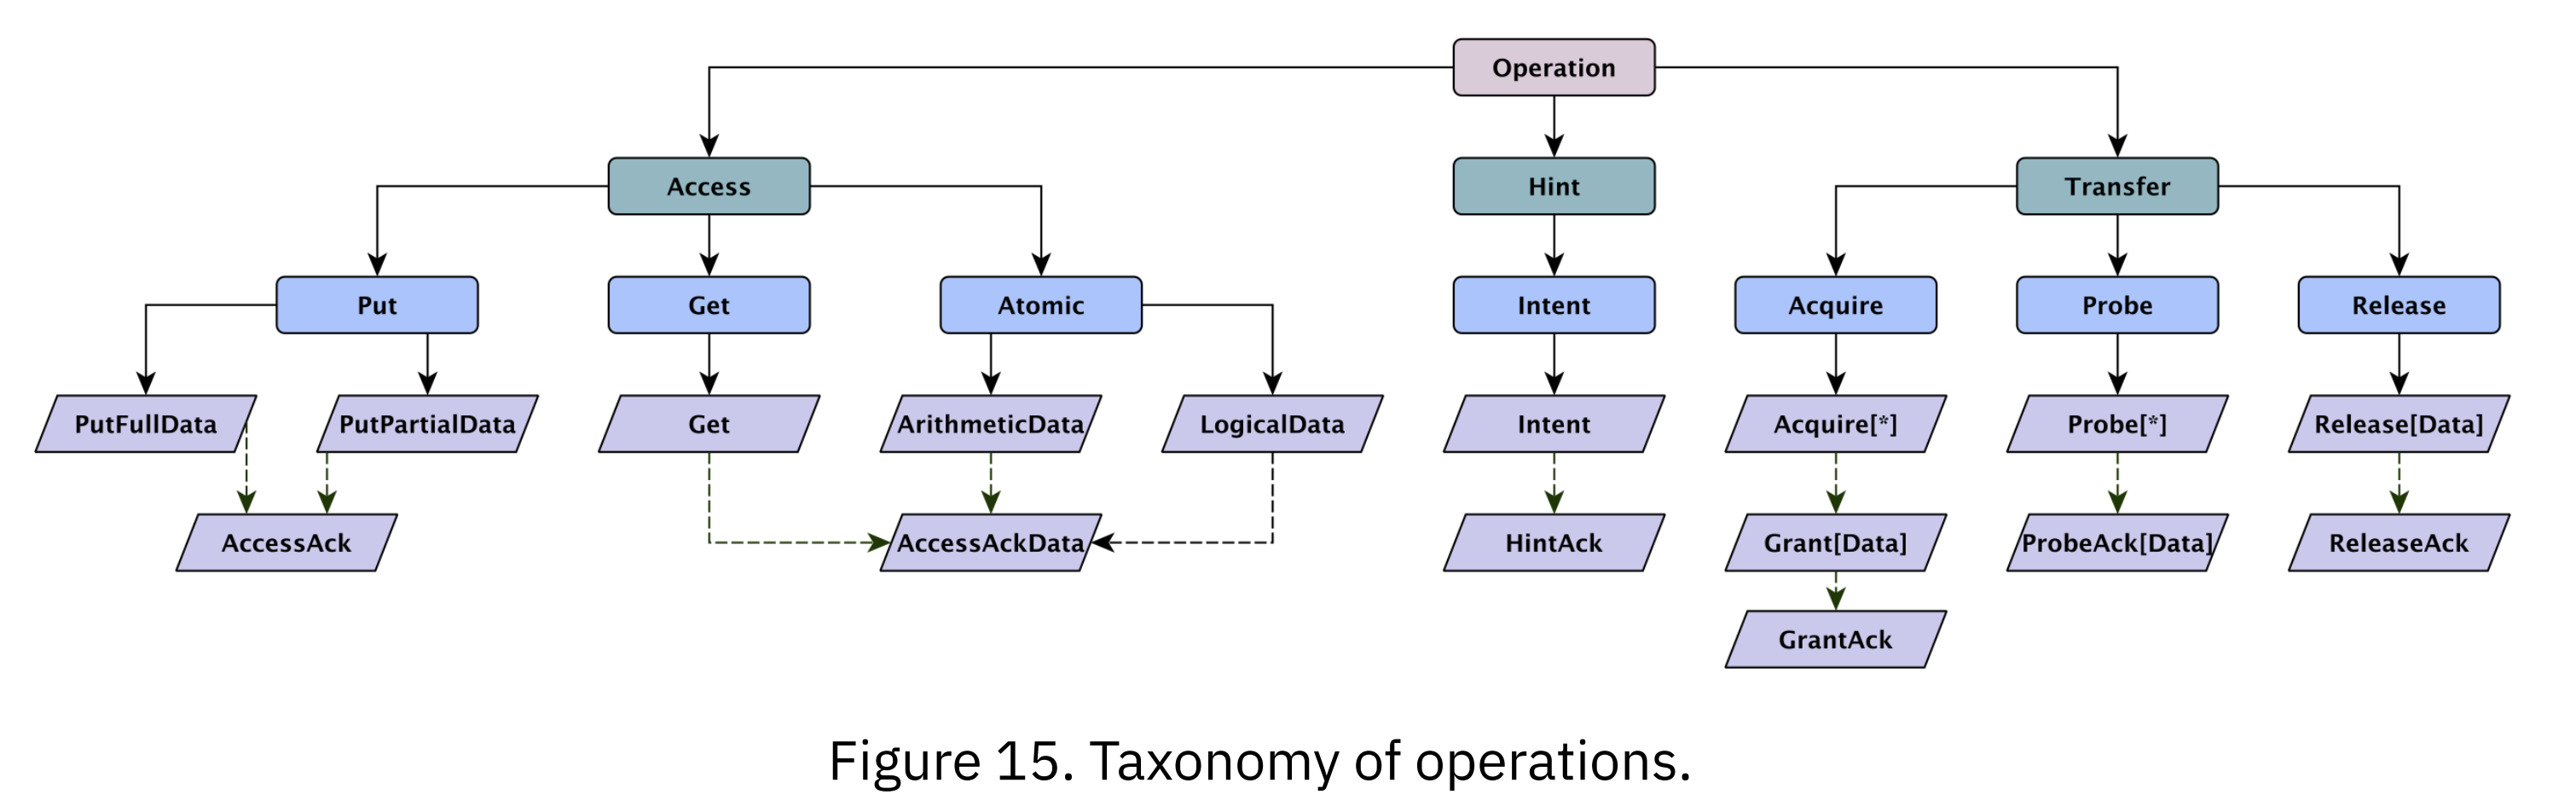
\includegraphics[width=\textwidth]{Img/TileLink_Operations.PNG} %插入图片,[]中设置图片大小,{}中是图片文件名
\caption{Taxonomy of operations} %最终文档中希望显示的图片标题
\label{TileLink_Operations} %用于文内引用的标签
\end{figure}

\paragraph{Get操作}
Get操作是master对slave发起uncache的读,master只需要数据,而不需要缓存这个数据的权限。Get操作请求由master通过A通道发送Get消息,确认信息由slave通过D通道发送AccessAckData消息。

\paragraph{Put操作}
Put操作是master对slave发起uncache的写,master只需要把新数据写进slave就可以了,而不需要缓存这个数据的权限。Put操作请求由master通过A通道发送PutFullData或者PutPartialData消息,确认信息由slave通过D通道发送AccessAck消息。

\paragraph{Acquire操作}
Acquire操作是master对slave发起的申请块权限的操作。当操作完成后,master将获得块的特定权限,它将可以将数据块缓存在本地,并在本地执行权限允许的读写操作。
Acquire操作包含三步:
\begin{enumerate}
	\item master向slave发送Acquire消息,对于特定数据块申请特定的权限。
	\item slave向master回复Grant[Data]消息,对于此数据块,赋予master特定的权限(此权限可能比master请求的权限更高)。
	\item master使用GrantAck响应消息来提供对事务完成的最终确认。
\end{enumerate}

\paragraph{Probe操作}
Probe操作是slave对master发起的块权限查询或修改操作。当操作完成后,master将失去块的部分或全部权限。
Probe操作包含两步:首先slave向master发送ProbeBlock或ProbePerm消息,表明它希望将master缓存的特定数据块的降至特定的权限。接着,master回复ProbeAck[Data]来确认此消息,并写回可能的脏数据。

\paragraph{Release操作}
Release操作是master对slave发起的,主动的释放块权限和数据的操作。当操作完成后,master将失去块的部分或全部权限。
Release操作包含两步:首先master向slave发送Release[Data]消息,表明它将自己缓存的特定数据块降至特定的权限,同时写回可能有的脏数据。接着,slave回复ReleaseAck来确定此消息。

\section{TileLink与一致性协议}

在前面的小节中,我们介绍了TileLink中有哪些通道,哪些消息,哪些操作,其中有些就是和维护一致性有关的。在这一小节,我们完整介绍TileLink协议是如何维护一致性的。包括TileLink定义的块的权限,权限的转移以及操作定序等。
TileLink定义了缓存的数据块的权限包括None,Read以及Read + Write。
在TileLink中,对于一个数据块的所有缓存将构成了一棵树。树的根节点都位于缓存数据块的最终存储位置,例如DDR。根据节点在树中的不同位置,可以划分为四类:
\begin{itemize}
	\item Nothing:当前不缓存数据副本的节点,没有读取或写入权限。
	\item Trunk:在Tip和根节点之间的路径上具有缓存副本的节点。这类节点既没有读权限也没有写权限。例如,当写权限位于L1时,其下面的L2和L3就位于L1到根节点DDR的路径上,L2和L3就处于Trunk状态。
	\item Tip:缓存了数据副本节点,拥有最高权限,是负责对读写请求序列化的点。此状态下拥有对其副本的读/写权限,其中可能包含脏数据。
	\item Branch:在Tip上方的具有缓存副本的节点。对其副本具有只读权限。
\end{itemize}

下面我们可以简单对比一下TileLink协议的状态和MESI的状态,上述四种状态,无法严格对应到MESI协议,但大部分是可以对应过去的。
MESI协议中有四种状态,分别是:
\begin{itemize}
	\item Modified (M)
	\item Exclusive (E)
	\item Shared (S)
	\item Invalid (I)
\end{itemize}

Nothing和Invalid,Branch和Shared是可以一一对应的。Tip对应于Modified和Exclusive状态。TileLink在设计上,并不需要其他节点区分拥有写权限的节点有没有修改过数据,是不是dirty的。它们只需要只需要知道那个节点拥有最高权限就可以。至于是否修改过数据,只有那个节点自己需要关心,拥有最高权限的节点,可以自己内部设计有dirty bit,来记录自己有没有修改过数据,并根据这个bit来判断自己要不要写回脏数据。
Trunk状态是TileLink所独有的,这与TileLink的一致性协议设计是有关的。TileLink要求对于任何一块被缓存的数据块,所有缓存了它的节点必须组成一棵树,称为coherence tree。由于TileLink网络是有向无环图,同时被缓存的数据块唯一来自一个根节点(如DDR),需要组成树,实际上要求下级cache对上一级cache保持Inclusive的关系。这并不是说TileLink要求所有的cache都必须被设计成Inclusive Cache。下一级Cache并不需要真的缓存这个数据块,但是它需要知道自己处于Trunk状态,并且自己的子节点缓存了这个块。

在TileLink的网络中,节点之间通过执行权限转移操作,保证了数据的一致性以及对数据写的定序。
一般来说:
Acquire操作用来主动申请权限。
而Release操作用来主动地降低权限(例如当cache发生了替换,需要写时)。
Probe操作是一致性的invalidate请求,用来降低client的权限。

下面我们以一组例子说明在TileLink网络中,一致性是如何维护的:
\begin{figure}[H] %H为当前位置,!htb为忽略美学标准,htbp为浮动图形
\centering %图片居中
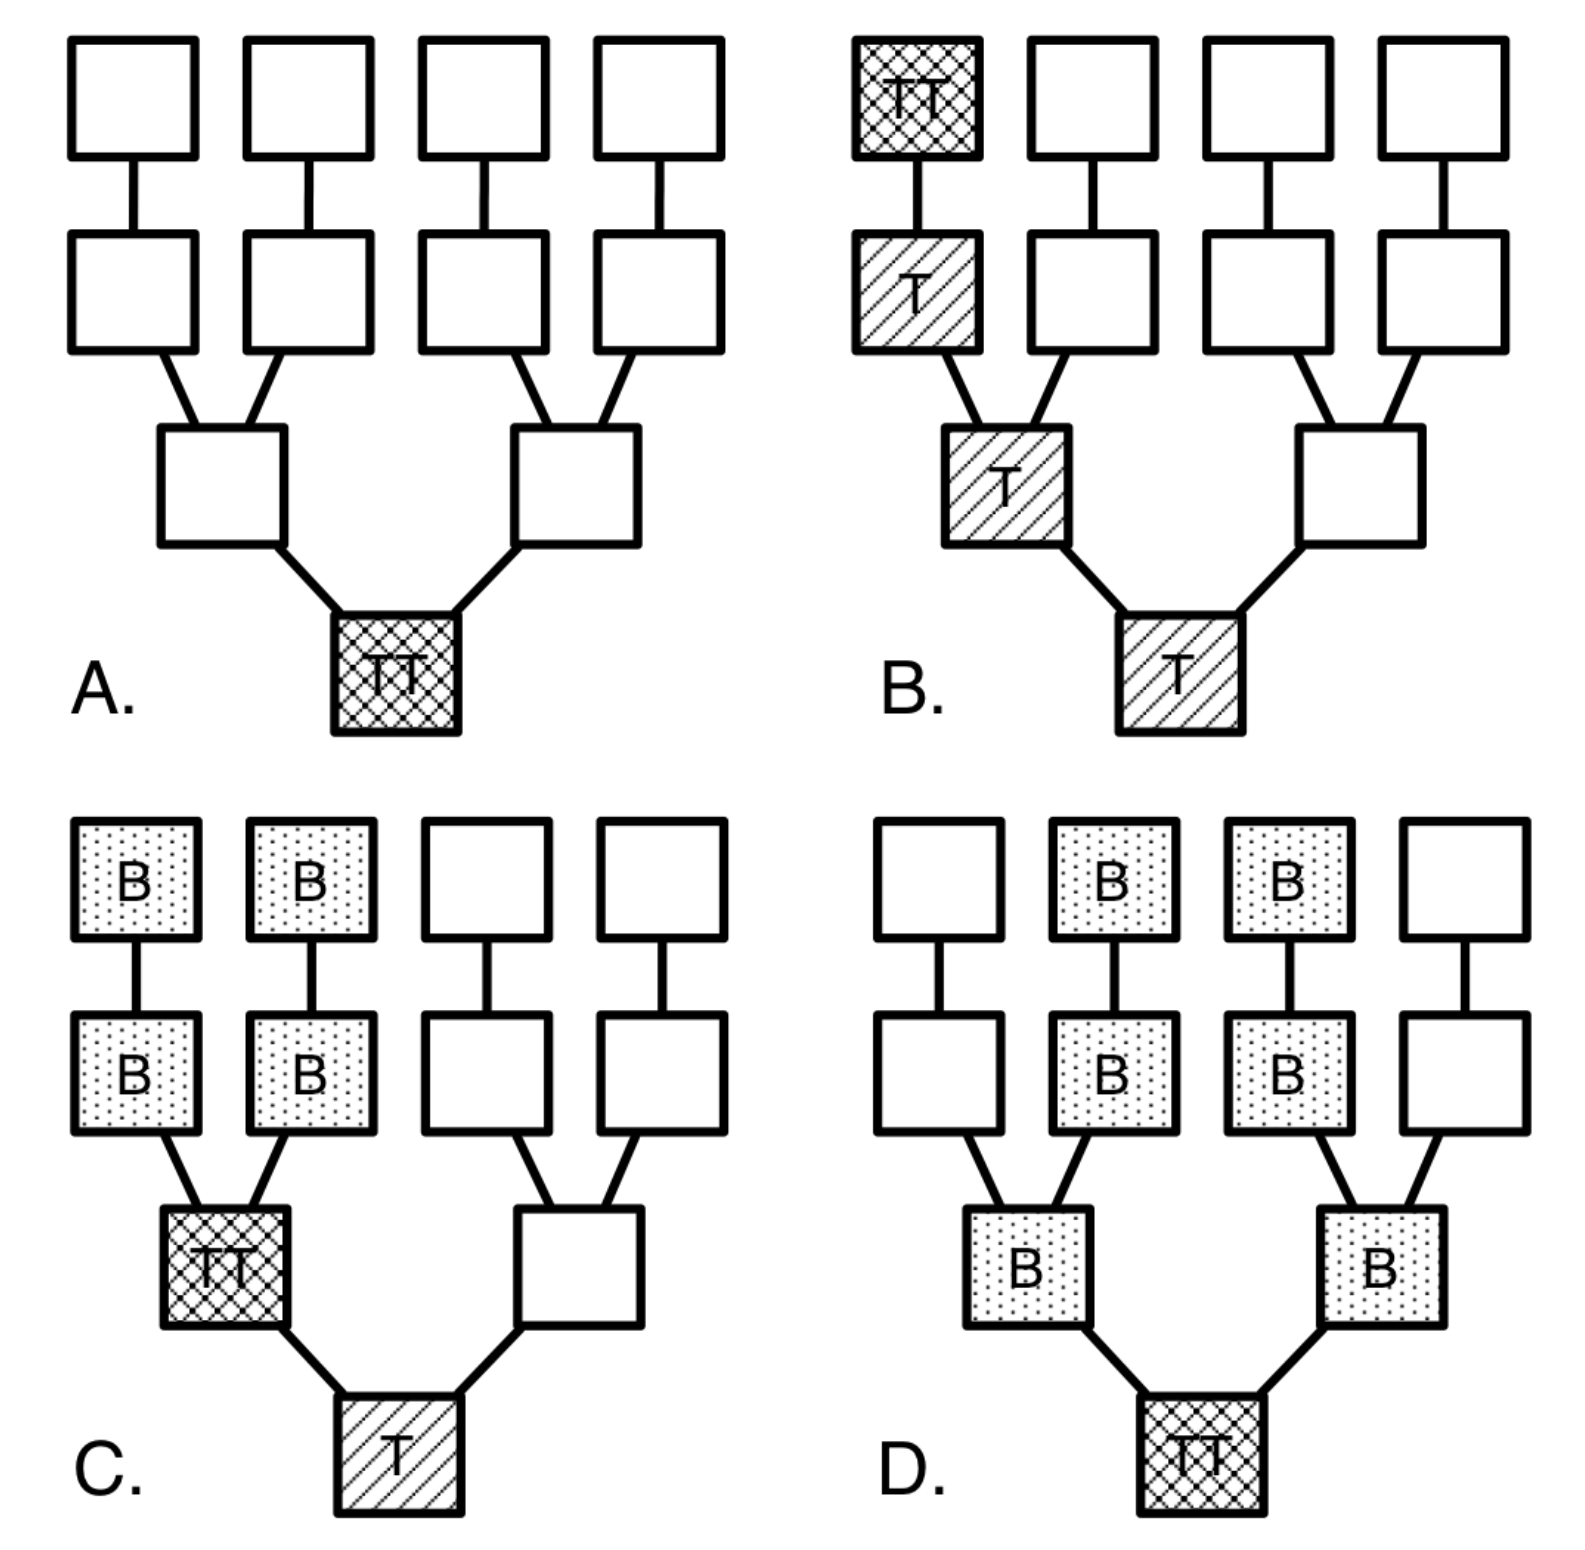
\includegraphics[width=\textwidth]{Img/TileLink_coherence.PNG} %插入图片,[]中设置图片大小,{}中是图片文件名
\caption{TileLink coherence examples} %最终文档中希望显示的图片标题
\label{TileLink_coherence} %用于文内引用的标签
\end{figure}

图中的树描述了一个系统中的多个缓存节点。最下方是DDR,最上方是L1 Cache。缓存了某个特定数据块的所有缓存节点构成了一棵树,以DDR为树根。
假设这是针对某个数据块d1的coherence tree。
图中的状态标识是:空白指Nothing状态,B指Branch状态,T指Trunk状态,TT是Tip状态。
L1 Cache从左到右标号分别为0,1,2,3。
L2 Cache从左到右标号分别为0,1,2,3。
L3 Cache从左到右标号分别为0,1。

图A到D,展示了系统中针对数据块d1的coherence tree的变化过程。

\begin{enumerate}
	\item 开始时,在图A的状态下,数据块d1存在于DDR中,系统中的其他cache都没有缓存d1,因此DDR节点是TT状态。
	\item L1 0请求了d1的写权限,因此从L1 0开始逐级向下通过Acquire操作升级权限,最终Tip状态从DDR转移到了L1 Cache 0,路径上的其他节点都变成了Trunk状态。Coherence Tree演化为了图B状态。
	\item L1 1通过Acquire申请d1的读权限,L2 1也向下转发请求,Acquire请求到达L3 0。L3 0发现自己处于Trunk状态,意味着它的某个孩子节点拥有Tip状态。因此L3 0向L2 0发送ProbeBlock请求,L2 0发现自己也是Trunk状态,因此将ProbeBlock向上发送到L1 0。L1 0收到ProbeBlock请求后,通过ProbeAckData消息将自己的权限降为Branch,并将脏数据写回到L2 0。L2 0也将ProbeAckData发送到L3 0,L2 0变为Branch状态。L3 0收到ProbeAckData后,回收了针对d1数据块的Tip权限,并通过GrantData,将数据和权限发送到L2 1,进而上传到L1 1,它们变为了Branch状态。Coherence Tree演化到了图C状态。
	\item L1 2通过Acquire申请d1的读权限,与前一步一样,最终Tip权限回到了DDR。值得注意的是,在图D中,L1 0和L2 0的Branch状态消失了,这不是L1 2的读导致的,可能是它们自己释放导致的。最终,Coherence Tree演化为了图D。
\end{enumerate}

\section{Verification}

随着系统复杂性的提升,流片成本的增加,如何保证芯片设计实现完整地达到功能与性能要求,没有设计或实现的漏洞,成为了非常关键的问题。验证应运而生。功能验证是在流片前验证开发设计是否遵守给定规格的工作,在芯片全流程中占据关键位置。如今,验证是设计过程中的基本步骤,它比设计实现需要更高的资源,甚至高达30%到40%的项目资源。

本节介绍功能验证的基本流程以及基本方法。

\subsection{Verification的基础知识}

\subsubsection{验证在芯片开发中的位置}

验证主要是验证硬件设计开发是否遵守给定的规格,在整个芯片设计流程中居于关键的位置。
下图展示了芯片硅前开发流程:
\begin{figure}[H] %H为当前位置,!htb为忽略美学标准,htbp为浮动图形
\centering %图片居中
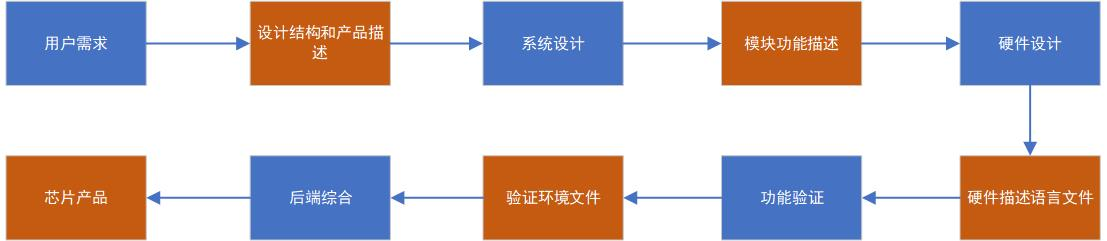
\includegraphics[width=\textwidth]{Img/芯片硅前开发流程.jpg} %插入图片,[]中设置图片大小,{}中是图片文件名
\caption{芯片硅前开发流程} %最终文档中希望显示的图片标题
\label{芯片硅前开发流程} %用于文内引用的标签
\end{figure}

可以看到芯片验证位于硬件描述产出之后,负责根据设计结构和产品详述以及模块功能详述,对产出的硬件设计进行验证。
一般来说,当细分模块初步完成RTL设计后,验证团队要做几项工作来检查设计:
\begin{enumerate}
	\item 设计文件是否正确地按照功能描述文档实施了?
	\item 硬件设计人员是否有遗漏掉的边界情况(Corner Case)?
\end{enumerate}

我感觉这一部分可以去掉。大家不用知道这种琐碎的细节。
在实际项目中,硬件设计人员和功能验证人员的合作是紧密的,如下图所示:
\begin{figure}[H] %H为当前位置,!htb为忽略美学标准,htbp为浮动图形
\centering %图片居中
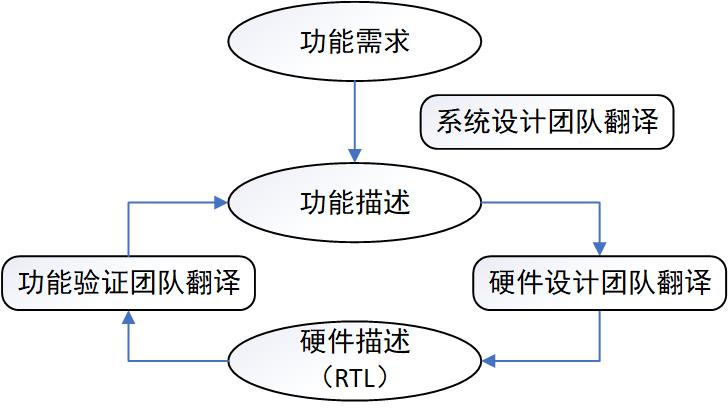
\includegraphics[width=\textwidth]{Img/设计和验证团队协同工作示意图.jpg} %插入图片,[]中设置图片大小,{}中是图片文件名
\caption{设计和验证团队协同工作示意图} %最终文档中希望显示的图片标题
\label{设计和验证团队协同工作示意图} %用于文内引用的标签
\end{figure}

\begin{enumerate}
	\item 当系统设计团队将功能需求(抽象指标)翻译为功能描述(自然语言)之后,硬件设计团队和功能验证团队要围绕功能描述文档分别展开各自的工作。
	\item 当设计团队初步实现设计以后,验证团队要搭建验证环境展开各功能点的验证。
	\item 当验证环境测试出的结果与预期不符时,如果是设计与功能描述存在明显不符,则应该更改设计。如果是功能描述描述不清或者存在漏洞,则应修改功能描述,确保双方对功能描述理解一致。
\end{enumerate}

\subsubsection{功能验证的完备周期}

下图展示了功能验证的一个完整周期。

\begin{enumerate}
	\item 首先是系统工程师给出的功能详述文档。对于每一个芯片,大到芯片自身,小到细分的模块,都需要有功能详述文档。功能详述文档详细描述了,接口信息、结构信息、交互信息等。
	\item 接着就需要制定验证计划,验证计划一般包括验证方法、验证工具、验证完备标准、验证资源、需要验证的功能点等。
	\item 开发验证环境
	\item 调试环境和HDL文件。通过测试硬件设计,来发现验证环境的瑕疵以及HDL实现的问题。
	\item 回归测试:每当硬件修复了缺陷或者添加了某项新功能后,都需要通过测试用例,来验证硬件的正确性。
	\item 芯片生产:当所有的验证都通过,并完成了后端工作后,芯片将投片生产。
	\item 硅后系统测试:当芯片返回后,测试人员依照系统集成的顺序,从底层模块开始测试。
	\item 逃逸分析:凡是硅后系统测试发现的bug,都是从验证时期逃脱掉的。我们需要分析此bug没有被测试到的原因,并完善验证测试用例,防止下次再出现类似的问题。
\end{enumerate}

\begin{figure}[H] %H为当前位置,!htb为忽略美学标准,htbp为浮动图形
\centering %图片居中
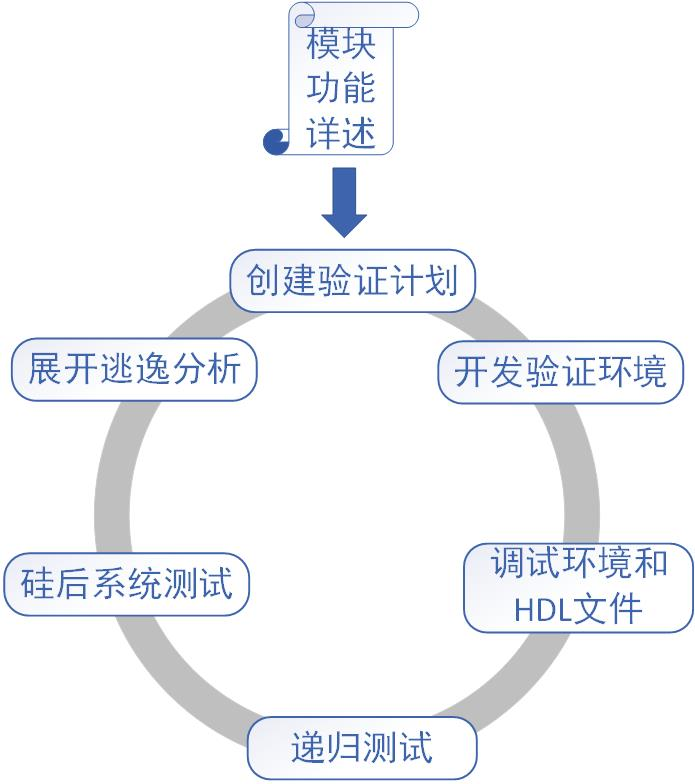
\includegraphics[width=0.5\textwidth]{Img/功能验证的完备周期.jpg} %插入图片,[]中设置图片大小,{}中是图片文件名
\caption{功能验证的完备周期} %最终文档中希望显示的图片标题
\label{功能验证的完备周期} %用于文内引用的标签
\end{figure}

\subsubsection{功能验证的方法}

随着设计的复杂化,到了目前的阶段,我们已经无法依赖单一的工具、语言或方法来达到验证的完备性。在实践中,大家发展了许多中不同的方法,我们需要根据需求选用合适的方法,并进行合适的组合,才能达到完备的验证。目前主流的验证方法包括:动态仿真与静态检查。

\paragraph{动态仿真}

动态仿真是通过测试序列和激励生成器给待验证设计适当的激励,随着仿真进程的推进,判断输出是否符合预期。按照激励生成的方式和检查方式,可以将动态仿真进一步划分为:
\begin{itemize}
	\item 定向测试:指激励内容在运行之前已经确定下来,每次运行的激励序列都是一样的。定向测试一般应用在模块测试的早期或者系统级芯片测试场景中,它适合于测试设计的基本功能。
	\item 随机测试:随机测试通过预先定义的约束,每次随机产生出合理的数值,通过激励发生器给出测试序列。约束实际上是决定随机激励能否符合接口协议的关键,也是朝向验证合理状态空间的关键。目前常用的一种随机验证方式是基于覆盖率驱动的。在每次测试中我们都收集覆盖率,根据这些反馈来缩窄随机约束域,使其偏置产生一些序列,覆盖那些没有被现有随机测试覆盖到的功能点。
	\item 断言检查:设计人员或验证人员在运行时假如各种各样的断言(assertion),它可以用于对某一特定的逻辑或时序进行预设,一旦设计的实际行为不符合断言的描述,则给出检查报告。
\end{itemize}

\paragraph{静态检查}

与动态仿真相对应的是静态检查,它本身不需要仿真、波形激励,验证人员通过工具的辅助即可以发现设计中存在的问题。

\begin{itemize}
	\item 语法检查
	\item 语义检查:例如检查寄存器未初始化,X值的传播等。
	\item 跨时钟域检查
	\item 形式验证:在动态仿真验证中,我们是通过生成各种测试序列来访问设计中的状态的。在理论上,所有可以跳转的设计状态总和被称为可及状态空间。形式验证可以通过数学的方法遍历状态空间,进而证明设计行为符合属性描述。在遍历过程中,一旦遇到反例,形式验证工具就会停下来。形式验证通常对较小规模的电路具有很好的效果。而对于较大规模的电路,稍微复杂一点的模块,形式验证则无法进行有效的验证。
\end{itemize}

\subsection{UVM验证方法学}

UVM(Universal Verification Methodology )是一种常用的,基于动态仿真的验证方法学。UVM是一种事务级方法(transaction-level methodology (TLM)),利用这个方法,我们可以生成仿真的激励。
UVM通用用诸如SystemVerilog的面向对象编程(OOP)语言实现,这些语言提供了广泛的类和库,可轻松开发可重复使用的且功能强大的测试。
特别是,它提供的库和模型使工程师能够创建任何所需的结构并提供接口以便事务级别进行连接。

最重要的是,UVM已经成为进行有效且详尽的验证的事实标准与最佳实践。UVM是基于SystemVerilog语言,并定义了一套用于测试DUT的结构。最基本的UVM结构如下图所示。本节的目当然不是精确描述UVM语言,它是一门完整的编程语言并且需要好几本书来恰当地讲解。在这里,我们想要简要地介绍经典的UVM结构,因为这是本验证工作的一个核心基础。如图XXX所示,经典的UVM验证包括如下模块:

\begin{itemize}
	\item Test:Test是最顶层的UVM组件,它实例化并配置了整个验证环境。
	\item Environment:将所有针对DUT的组件组合在一起。它定义了UVM测试的可重用组件拓扑。
	\item Agent:代理包含UVM结构的大多数模块,例如:
		\begin{itemize}
			\item Sequencer:创建事务并将其发送到Driver的定序器。
			\item Driver:接收sequence items并把它们通过虚拟接口发送到DUT。
			\item Monitor:将输入和输出数据通过虚拟接口收集上来,并发送到计分板检查DUT的输出是否正确。
		\end{itemize}
\end{itemize}

\begin{figure}[H] %H为当前位置,!htb为忽略美学标准,htbp为浮动图形
\centering %图片居中
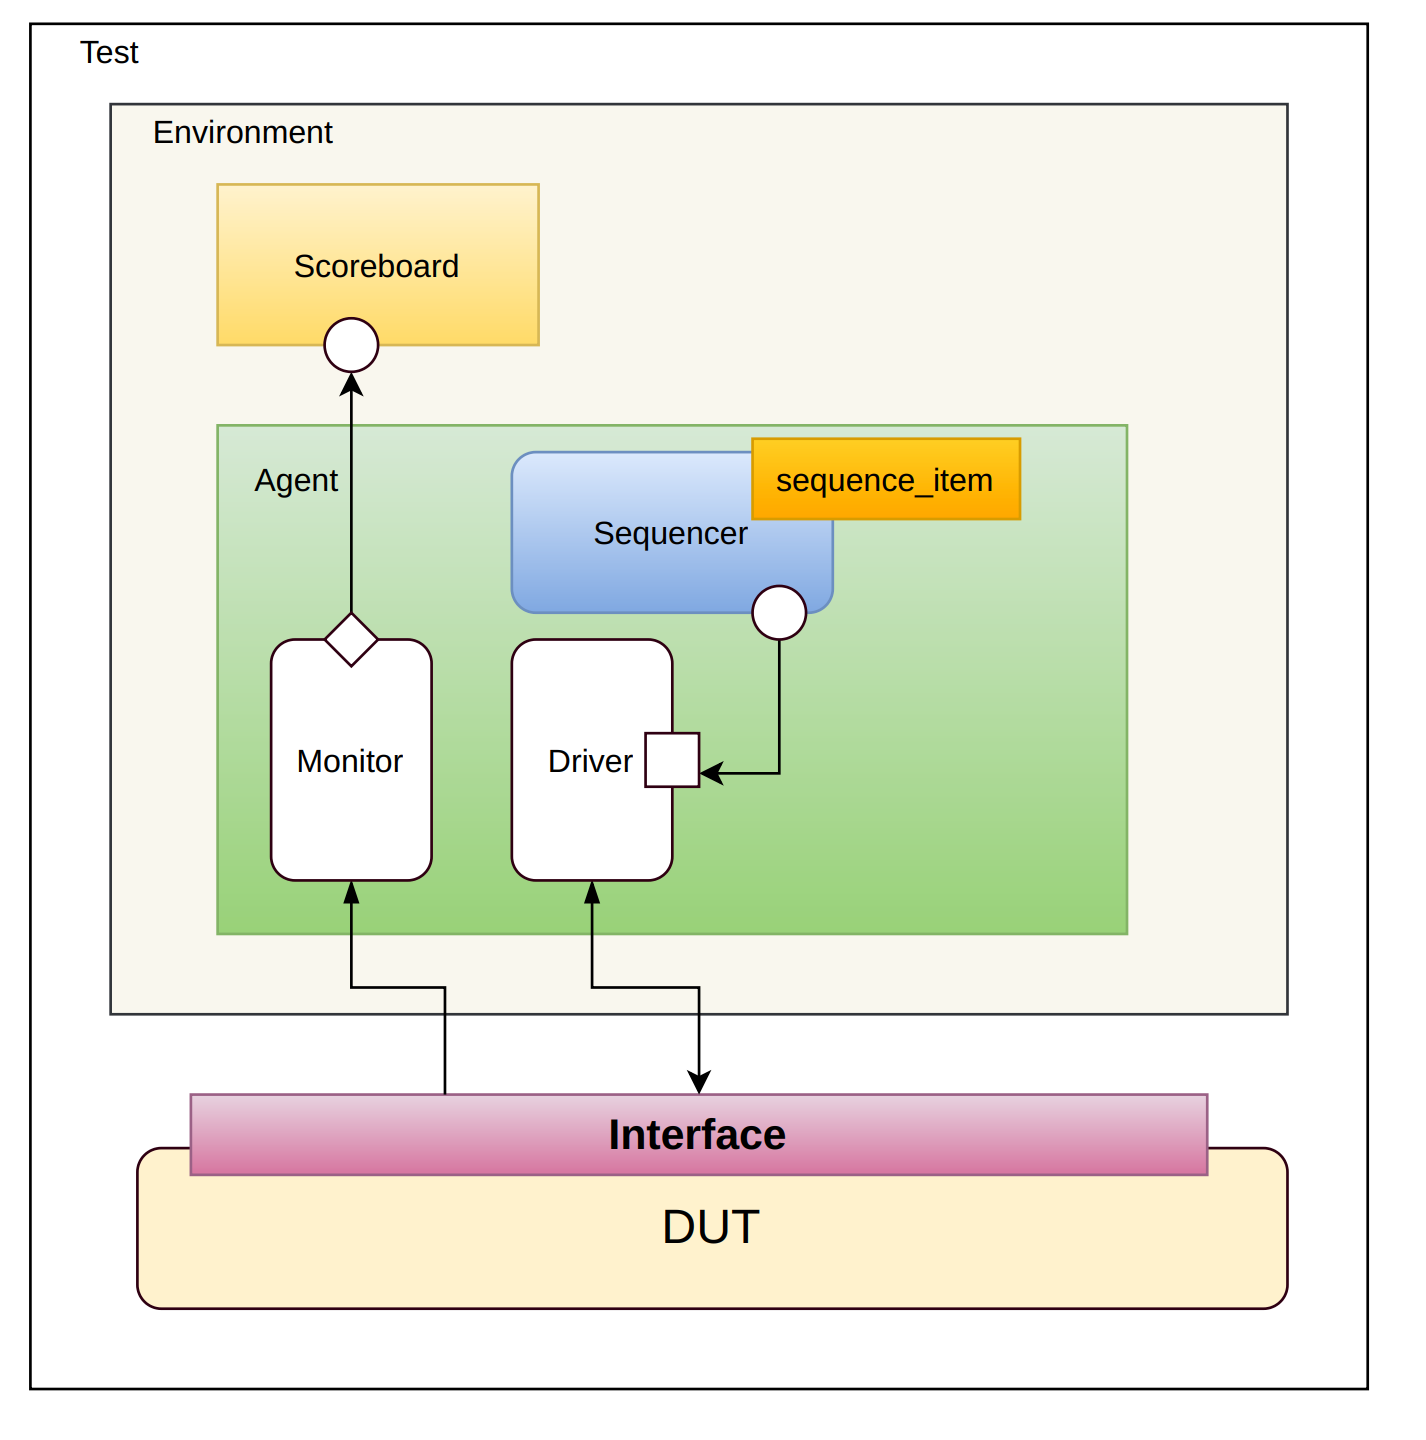
\includegraphics[width=0.5\textwidth]{Img/UVM的基本结构.PNG} %插入图片,[]中设置图片大小,{}中是图片文件名
\caption{UVM的基本结构} %最终文档中希望显示的图片标题
\label{UVM的基本结构} %用于文内引用的标签
\end{figure}

UVM的强大之处是可重用性和易用性:可重用性是通过override实例化对象的类来实现的。我们唯一需要考虑的就是测试,而不是编写UVM代码结构。UVM代码框架始终是标准的,并具有很高的模块化性。这大大地减少了验证时间,并让UVM真正成为了通用的验证的标准。
